% Options for packages loaded elsewhere
\PassOptionsToPackage{unicode}{hyperref}
\PassOptionsToPackage{hyphens}{url}
%
\documentclass[
]{article}
\usepackage{lmodern}
\usepackage{amssymb,amsmath}
\usepackage{ifxetex,ifluatex}
\ifnum 0\ifxetex 1\fi\ifluatex 1\fi=0 % if pdftex
  \usepackage[T1]{fontenc}
  \usepackage[utf8]{inputenc}
  \usepackage{textcomp} % provide euro and other symbols
\else % if luatex or xetex
  \usepackage{unicode-math}
  \defaultfontfeatures{Scale=MatchLowercase}
  \defaultfontfeatures[\rmfamily]{Ligatures=TeX,Scale=1}
\fi
% Use upquote if available, for straight quotes in verbatim environments
\IfFileExists{upquote.sty}{\usepackage{upquote}}{}
\IfFileExists{microtype.sty}{% use microtype if available
  \usepackage[]{microtype}
  \UseMicrotypeSet[protrusion]{basicmath} % disable protrusion for tt fonts
}{}
\makeatletter
\@ifundefined{KOMAClassName}{% if non-KOMA class
  \IfFileExists{parskip.sty}{%
    \usepackage{parskip}
  }{% else
    \setlength{\parindent}{0pt}
    \setlength{\parskip}{6pt plus 2pt minus 1pt}}
}{% if KOMA class
  \KOMAoptions{parskip=half}}
\makeatother
\usepackage{xcolor}
\IfFileExists{xurl.sty}{\usepackage{xurl}}{} % add URL line breaks if available
\IfFileExists{bookmark.sty}{\usepackage{bookmark}}{\usepackage{hyperref}}
\hypersetup{
  pdftitle={Computing in Oceanography: data visualization},
  hidelinks,
  pdfcreator={LaTeX via pandoc}}
\urlstyle{same} % disable monospaced font for URLs
\usepackage[margin=1in]{geometry}
\usepackage{color}
\usepackage{fancyvrb}
\newcommand{\VerbBar}{|}
\newcommand{\VERB}{\Verb[commandchars=\\\{\}]}
\DefineVerbatimEnvironment{Highlighting}{Verbatim}{commandchars=\\\{\}}
% Add ',fontsize=\small' for more characters per line
\usepackage{framed}
\definecolor{shadecolor}{RGB}{248,248,248}
\newenvironment{Shaded}{\begin{snugshade}}{\end{snugshade}}
\newcommand{\AlertTok}[1]{\textcolor[rgb]{0.94,0.16,0.16}{#1}}
\newcommand{\AnnotationTok}[1]{\textcolor[rgb]{0.56,0.35,0.01}{\textbf{\textit{#1}}}}
\newcommand{\AttributeTok}[1]{\textcolor[rgb]{0.77,0.63,0.00}{#1}}
\newcommand{\BaseNTok}[1]{\textcolor[rgb]{0.00,0.00,0.81}{#1}}
\newcommand{\BuiltInTok}[1]{#1}
\newcommand{\CharTok}[1]{\textcolor[rgb]{0.31,0.60,0.02}{#1}}
\newcommand{\CommentTok}[1]{\textcolor[rgb]{0.56,0.35,0.01}{\textit{#1}}}
\newcommand{\CommentVarTok}[1]{\textcolor[rgb]{0.56,0.35,0.01}{\textbf{\textit{#1}}}}
\newcommand{\ConstantTok}[1]{\textcolor[rgb]{0.00,0.00,0.00}{#1}}
\newcommand{\ControlFlowTok}[1]{\textcolor[rgb]{0.13,0.29,0.53}{\textbf{#1}}}
\newcommand{\DataTypeTok}[1]{\textcolor[rgb]{0.13,0.29,0.53}{#1}}
\newcommand{\DecValTok}[1]{\textcolor[rgb]{0.00,0.00,0.81}{#1}}
\newcommand{\DocumentationTok}[1]{\textcolor[rgb]{0.56,0.35,0.01}{\textbf{\textit{#1}}}}
\newcommand{\ErrorTok}[1]{\textcolor[rgb]{0.64,0.00,0.00}{\textbf{#1}}}
\newcommand{\ExtensionTok}[1]{#1}
\newcommand{\FloatTok}[1]{\textcolor[rgb]{0.00,0.00,0.81}{#1}}
\newcommand{\FunctionTok}[1]{\textcolor[rgb]{0.00,0.00,0.00}{#1}}
\newcommand{\ImportTok}[1]{#1}
\newcommand{\InformationTok}[1]{\textcolor[rgb]{0.56,0.35,0.01}{\textbf{\textit{#1}}}}
\newcommand{\KeywordTok}[1]{\textcolor[rgb]{0.13,0.29,0.53}{\textbf{#1}}}
\newcommand{\NormalTok}[1]{#1}
\newcommand{\OperatorTok}[1]{\textcolor[rgb]{0.81,0.36,0.00}{\textbf{#1}}}
\newcommand{\OtherTok}[1]{\textcolor[rgb]{0.56,0.35,0.01}{#1}}
\newcommand{\PreprocessorTok}[1]{\textcolor[rgb]{0.56,0.35,0.01}{\textit{#1}}}
\newcommand{\RegionMarkerTok}[1]{#1}
\newcommand{\SpecialCharTok}[1]{\textcolor[rgb]{0.00,0.00,0.00}{#1}}
\newcommand{\SpecialStringTok}[1]{\textcolor[rgb]{0.31,0.60,0.02}{#1}}
\newcommand{\StringTok}[1]{\textcolor[rgb]{0.31,0.60,0.02}{#1}}
\newcommand{\VariableTok}[1]{\textcolor[rgb]{0.00,0.00,0.00}{#1}}
\newcommand{\VerbatimStringTok}[1]{\textcolor[rgb]{0.31,0.60,0.02}{#1}}
\newcommand{\WarningTok}[1]{\textcolor[rgb]{0.56,0.35,0.01}{\textbf{\textit{#1}}}}
\usepackage{graphicx,grffile}
\makeatletter
\def\maxwidth{\ifdim\Gin@nat@width>\linewidth\linewidth\else\Gin@nat@width\fi}
\def\maxheight{\ifdim\Gin@nat@height>\textheight\textheight\else\Gin@nat@height\fi}
\makeatother
% Scale images if necessary, so that they will not overflow the page
% margins by default, and it is still possible to overwrite the defaults
% using explicit options in \includegraphics[width, height, ...]{}
\setkeys{Gin}{width=\maxwidth,height=\maxheight,keepaspectratio}
% Set default figure placement to htbp
\makeatletter
\def\fps@figure{htbp}
\makeatother
\setlength{\emergencystretch}{3em} % prevent overfull lines
\providecommand{\tightlist}{%
  \setlength{\itemsep}{0pt}\setlength{\parskip}{0pt}}
\setcounter{secnumdepth}{-\maxdimen} % remove section numbering

\title{Computing in Oceanography: data visualization}
\author{}
\date{\vspace{-2.5em}}

\begin{document}
\maketitle

An important aspect of a scientist's job is how to present or visualize
their data. The goal is to \textbf{display information as clearly and
simply as possible}.

Yesterday, we used an online plotting tool (Tuva) to make oceanographic
profile plots. It was interactive, and fun to use, but there were some
problems with it:

\begin{enumerate}
\def\labelenumi{\arabic{enumi}.}
\tightlist
\item
  Pre-prepared and formatted dataset
\item
  Limited plotting options
\item
  Reproducibility
\end{enumerate}

Excel or Google Sheets are platforms scientists use to do data
visualization and analysis, but they can still have the same limitations
as above, especially when we start to work with \textbf{a lot} of data.
Often scientists in oceanography have a lot of data to deal with, and
using computing and programming tools are becomming an indispensible
part of doing science.

\hypertarget{todays-goal-learn-how-to-plot-oceanographic-profiles-using-the-computing-language-r}{%
\paragraph{\texorpdfstring{\textbf{Today's Goal: learn how to plot
oceanographic profiles using the computing language
R}}{Today's Goal: learn how to plot oceanographic profiles using the computing language R}}\label{todays-goal-learn-how-to-plot-oceanographic-profiles-using-the-computing-language-r}}

\hypertarget{set-up}{%
\subsubsection{Set-up}\label{set-up}}

\begin{enumerate}
\def\labelenumi{\arabic{enumi}.}
\tightlist
\item
  Create a folder on your computer for the Computing in Oceanography
  work \emph{don't use spaces in the name!}
  e.g.~\texttt{Jterm2020-computingInOceanography}
\item
  Create a subfolder (i.e.~a folder within that folder) for today's
  class e.g.~\texttt{dataVisualization} (\emph{again, no spaces!})
\end{enumerate}

\hypertarget{introduction-to-r}{%
\subsection{Introduction to R}\label{introduction-to-r}}

\hypertarget{installing-r-and-rstudio}{%
\subsubsection{Installing R and
RStudio}\label{installing-r-and-rstudio}}

\begin{enumerate}
\def\labelenumi{\arabic{enumi}.}
\item
  Install R program at: \url{http://cran.rstudio.com/} . This site has
  options for download for Linux, Mac, and Windows
\item
  Install r-studio (R interface)
  \url{http://www.rstudio.com/products/rstudio/download/} . Under
  ``installers'' you should see options for Mac and Windows
\end{enumerate}

\hypertarget{r-basics}{%
\subsubsection{R Basics}\label{r-basics}}

\hypertarget{rstudio}{%
\paragraph{RStudio}\label{rstudio}}

RStudio is a program to help you use R. You can write a bunch of R
commands in a \emph{script}, you can access help and documentation, you
can see any plots you make.

\hypertarget{set-a-working-directory}{%
\paragraph{Set a working directory}\label{set-a-working-directory}}

At the start of a sesssion, set the working directory:

\begin{Shaded}
\begin{Highlighting}[]
\KeywordTok{setwd}\NormalTok{(}\StringTok{'V://Catherine//Teaching//MSSM//Jterm2020//Jterm2020-computingInOceanography//dataVisualization//'}\NormalTok{)                                               }
\end{Highlighting}
\end{Shaded}

Note: You will get error message if folder does not exist.

\hypertarget{use-r-as-a-calculator}{%
\paragraph{Use R as a calculator}\label{use-r-as-a-calculator}}

\begin{Shaded}
\begin{Highlighting}[]
\DecValTok{5}\OperatorTok{+}\DecValTok{6}
\end{Highlighting}
\end{Shaded}

\begin{verbatim}
## [1] 11
\end{verbatim}

\begin{Shaded}
\begin{Highlighting}[]
\DecValTok{5}\OperatorTok{*}\DecValTok{6}
\end{Highlighting}
\end{Shaded}

\begin{verbatim}
## [1] 30
\end{verbatim}

\begin{Shaded}
\begin{Highlighting}[]
\DecValTok{5}\OperatorTok{/}\DecValTok{6}
\end{Highlighting}
\end{Shaded}

\begin{verbatim}
## [1] 0.8333333
\end{verbatim}

\hypertarget{objects}{%
\paragraph{Objects}\label{objects}}

You can assign values to an ``object'' (we call these \emph{numeric})
e.g.

\begin{Shaded}
\begin{Highlighting}[]
\NormalTok{x <-}\StringTok{ }\DecValTok{5}
\NormalTok{y <-}\StringTok{ }\DecValTok{6}
\NormalTok{x}
\end{Highlighting}
\end{Shaded}

\begin{verbatim}
## [1] 5
\end{verbatim}

\begin{Shaded}
\begin{Highlighting}[]
\NormalTok{x }\OperatorTok{+}\StringTok{ }\NormalTok{y}
\end{Highlighting}
\end{Shaded}

\begin{verbatim}
## [1] 11
\end{verbatim}

\begin{Shaded}
\begin{Highlighting}[]
\NormalTok{y <-}\StringTok{ }\DecValTok{5}
\NormalTok{x }\OperatorTok{+}\StringTok{ }\NormalTok{y}
\end{Highlighting}
\end{Shaded}

\begin{verbatim}
## [1] 10
\end{verbatim}

You can also assign letters or words to an object (we call these
\emph{characters} or \emph{strings}) e.g.

\begin{Shaded}
\begin{Highlighting}[]
\NormalTok{day <-}\StringTok{ "Monday"}
\NormalTok{day}
\end{Highlighting}
\end{Shaded}

\begin{verbatim}
## [1] "Monday"
\end{verbatim}

\begin{Shaded}
\begin{Highlighting}[]
\NormalTok{month <-}\StringTok{ "January"}
\NormalTok{month}
\end{Highlighting}
\end{Shaded}

\begin{verbatim}
## [1] "January"
\end{verbatim}

You can have two objects together within another object e.g.

\begin{Shaded}
\begin{Highlighting}[]
\NormalTok{dayMonth <-}\StringTok{ }\KeywordTok{c}\NormalTok{(day,month)}
\NormalTok{dayMonth}
\end{Highlighting}
\end{Shaded}

\begin{verbatim}
## [1] "Monday"  "January"
\end{verbatim}

This combined object \texttt{dayMonth} is called a \emph{vector}, and
each object within the vector is known as an \emph{element}.

You can even mix up the types of objects, but the numeric is changed to
a character e.g.~

\begin{Shaded}
\begin{Highlighting}[]
\NormalTok{mixedObject <-}\StringTok{ }\KeywordTok{c}\NormalTok{(day,x,y,month)}
\NormalTok{mixedObject}
\end{Highlighting}
\end{Shaded}

\begin{verbatim}
## [1] "Monday"  "5"       "5"       "January"
\end{verbatim}

i.e.~the second and third elements within the mixedObject are no longer
numbers, they are characters.

\hypertarget{indexing}{%
\paragraph{Indexing}\label{indexing}}

If we have a vector, we can extract out one of the elements e.g.

\begin{Shaded}
\begin{Highlighting}[]
\NormalTok{mixedObject[}\DecValTok{4}\NormalTok{]}
\end{Highlighting}
\end{Shaded}

\begin{verbatim}
## [1] "January"
\end{verbatim}

Or we can extract however many elements we want, we just need to specify
the location (or \emph{index number}) of the element within the vector

\begin{Shaded}
\begin{Highlighting}[]
\NormalTok{mixedObject[}\KeywordTok{c}\NormalTok{(}\DecValTok{3}\NormalTok{,}\DecValTok{4}\NormalTok{)]}
\end{Highlighting}
\end{Shaded}

\begin{verbatim}
## [1] "5"       "January"
\end{verbatim}

There's lots of good resources online - \textbf{the internet is your
friend when programming}.

\hypertarget{plotting-an-oceanographic-profile}{%
\subsection{Plotting an oceanographic
profile}\label{plotting-an-oceanographic-profile}}

\hypertarget{initialization}{%
\paragraph{Initialization}\label{initialization}}

Launch R-studio and navigate to the directory you want to work in.

\begin{Shaded}
\begin{Highlighting}[]
\KeywordTok{setwd}\NormalTok{(}\StringTok{'V://Catherine//Teaching//MSSM//Jterm2020//Jterm2020-computingInOceanography//dataVisualization//'}\NormalTok{)  }
\end{Highlighting}
\end{Shaded}

\hypertarget{create-a-script}{%
\paragraph{Create a script}\label{create-a-script}}

We are going to write all of our commands within a \emph{script}. A
script is just a document that has a series of R commands, and when you
run it, all the commands are run in one go. It is \textbf{really useful}
for redoing analyses, or remaking plots, or just remembering what you
did yesterday.

\hypertarget{load-data}{%
\paragraph{Load data}\label{load-data}}

Download the \texttt{20170912station4.csv} file from the Google Drive,
located in:

\texttt{Computing\ in\ Oceanography\textbackslash{}Data}

Save this file in the folder we created at the start of this session
(i.e.~our working directory, where our script is saved).

To load the data into R, type the following command at the start of your
script:

\begin{Shaded}
\begin{Highlighting}[]
\NormalTok{DATA <-}\StringTok{ }\KeywordTok{read.csv}\NormalTok{(}\StringTok{'20170912station4.csv'}\NormalTok{)}
\end{Highlighting}
\end{Shaded}

The data contained in that file are loaded into a variable (or object)
called ``DATA'', but we didn't have to call the variable ``DATA''. We
could have called it something else, like ``STATION\_4'', ``X'', or
``Pinocchio''.

\hypertarget{aside-summary-of-data}{%
\paragraph{Aside: summary of data}\label{aside-summary-of-data}}

If you are interested in all the data, you can look at a summary of what
is in this variable.

\begin{Shaded}
\begin{Highlighting}[]
\KeywordTok{summary}\NormalTok{(DATA)}
\end{Highlighting}
\end{Shaded}

\begin{verbatim}
##       Date             Station     Depth.m        Temperature.C   
##  Min.   :20170912   Min.   :4   Min.   :  0.791   Min.   : 6.835  
##  1st Qu.:20170912   1st Qu.:4   1st Qu.: 22.797   1st Qu.: 7.321  
##  Median :20170912   Median :4   Median : 46.926   Median : 9.669  
##  Mean   :20170912   Mean   :4   Mean   : 52.258   Mean   : 9.858  
##  3rd Qu.:20170912   3rd Qu.:4   3rd Qu.: 84.284   3rd Qu.:11.236  
##  Max.   :20170912   Max.   :4   Max.   :106.927   Max.   :15.103  
##   Salinity.PSU   Density.kg.m..3      PAR          Fluorescence.mg.m..3
##  Min.   :31.62   Min.   :23.35   Min.   :  0.000   Min.   :0.1046      
##  1st Qu.:32.24   1st Qu.:24.58   1st Qu.:  0.000   1st Qu.:0.1527      
##  Median :32.30   Median :24.89   Median :  0.383   Median :0.2755      
##  Mean   :32.30   Mean   :24.83   Mean   : 60.088   Mean   :0.6058      
##  3rd Qu.:32.56   3rd Qu.:25.46   3rd Qu.: 22.500   3rd Qu.:0.5544      
##  Max.   :32.64   Max.   :25.58   Max.   :914.000   Max.   :2.9206      
##  Turbidity.NTU       Beam.1.m..1    OxygenConcentration.umole.kg..1
##  Min.   :0.000200   Min.   :6.441   Min.   :206.3                  
##  1st Qu.:0.000400   1st Qu.:6.550   1st Qu.:212.1                  
##  Median :0.000600   Median :6.802   Median :220.5                  
##  Mean   :0.001059   Mean   :6.904   Mean   :227.8                  
##  3rd Qu.:0.001800   3rd Qu.:7.255   3rd Qu.:250.6                  
##  Max.   :0.003400   Max.   :7.950   Max.   :264.8                  
##  OxygenSaturation
##  Min.   : 68.87  
##  1st Qu.: 71.49  
##  Median : 78.26  
##  Mean   : 81.49  
##  3rd Qu.: 91.86  
##  Max.   :102.79
\end{verbatim}

\hypertarget{plotting-the-oceanographic-profile.}{%
\paragraph{Plotting the oceanographic
profile.}\label{plotting-the-oceanographic-profile.}}

To plot temperature (column 3) against depth (column 4):

\begin{Shaded}
\begin{Highlighting}[]
\KeywordTok{plot}\NormalTok{(DATA[,}\DecValTok{4}\NormalTok{],}\OperatorTok{-}\NormalTok{DATA[,}\DecValTok{3}\NormalTok{])}
\end{Highlighting}
\end{Shaded}

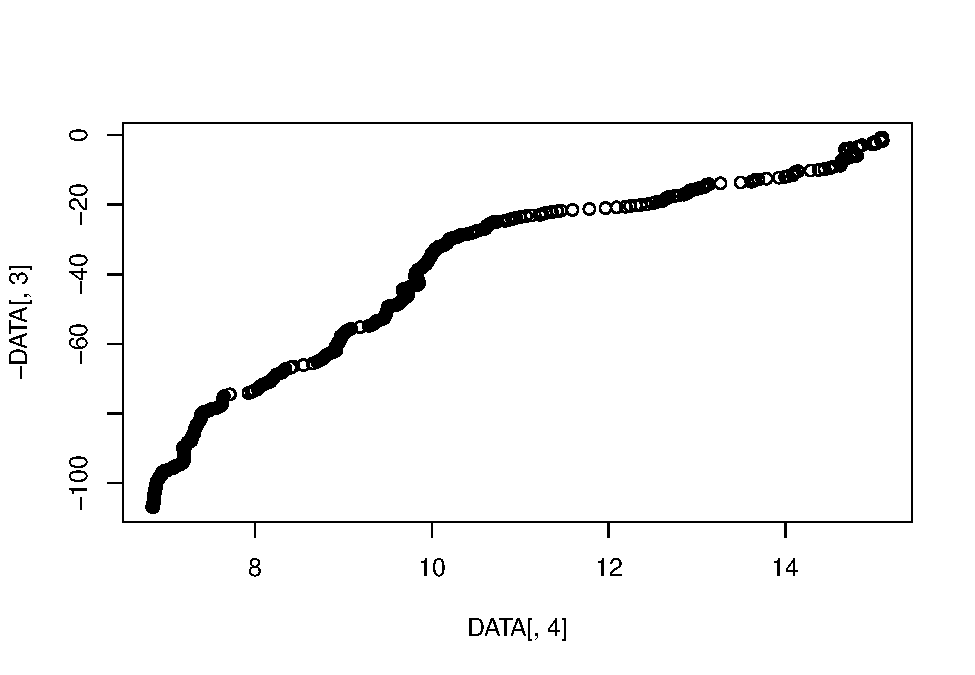
\includegraphics{dataVisualization-classNotes_files/figure-latex/unnamed-chunk-12-1.pdf}

Another option is to use the column headings instead of the column
numbers:

\begin{Shaded}
\begin{Highlighting}[]
\KeywordTok{plot}\NormalTok{(DATA[[}\StringTok{'Temperature.C'}\NormalTok{]],}\OperatorTok{-}\NormalTok{DATA[[}\StringTok{'Depth.m'}\NormalTok{]])}
\end{Highlighting}
\end{Shaded}

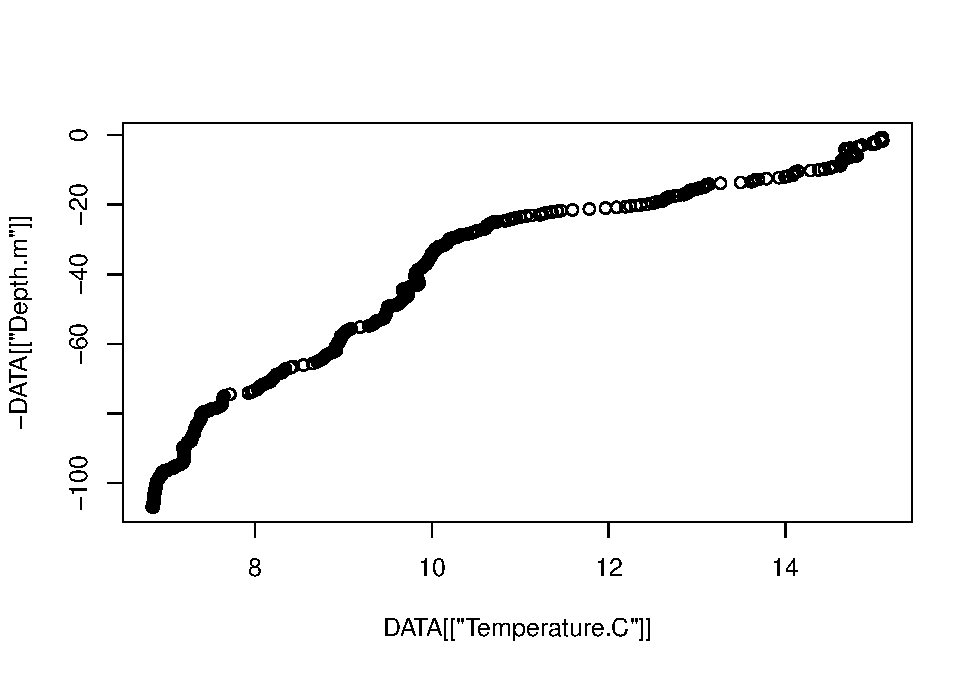
\includegraphics{dataVisualization-classNotes_files/figure-latex/unnamed-chunk-13-1.pdf}

\hypertarget{making-the-figure-nicer}{%
\paragraph{Making the figure nicer}\label{making-the-figure-nicer}}

There are lots of options to customize the figure, but for now, we are
just going to:

\begin{enumerate}
\def\labelenumi{\arabic{enumi}.}
\tightlist
\item
  label the axes (xlab, ylab)
\item
  set the axis limits (xlim, ylim)
\item
  plot the data as a line with dots (type)
\item
  set the color of the data (col)
\end{enumerate}

Add the following to your script:

\begin{Shaded}
\begin{Highlighting}[]
\KeywordTok{plot}\NormalTok{(DATA[[}\StringTok{'Temperature.C'}\NormalTok{]],}\OperatorTok{-}\NormalTok{DATA[[}\StringTok{'Depth.m'}\NormalTok{]],}
 \DataTypeTok{xlab=}\StringTok{'Temperature (deg C)'}\NormalTok{,}\DataTypeTok{ylab=}\StringTok{'Depth (m)'}\NormalTok{,}
 \DataTypeTok{xlim=}\KeywordTok{c}\NormalTok{(}\DecValTok{6}\NormalTok{,}\DecValTok{16}\NormalTok{),}\DataTypeTok{ylim=}\KeywordTok{c}\NormalTok{(}\OperatorTok{-}\DecValTok{110}\NormalTok{,}\DecValTok{0}\NormalTok{),}
 \DataTypeTok{type=}\StringTok{"b"}\NormalTok{,}\DataTypeTok{col=}\StringTok{"turquoise"}\NormalTok{)}
\end{Highlighting}
\end{Shaded}

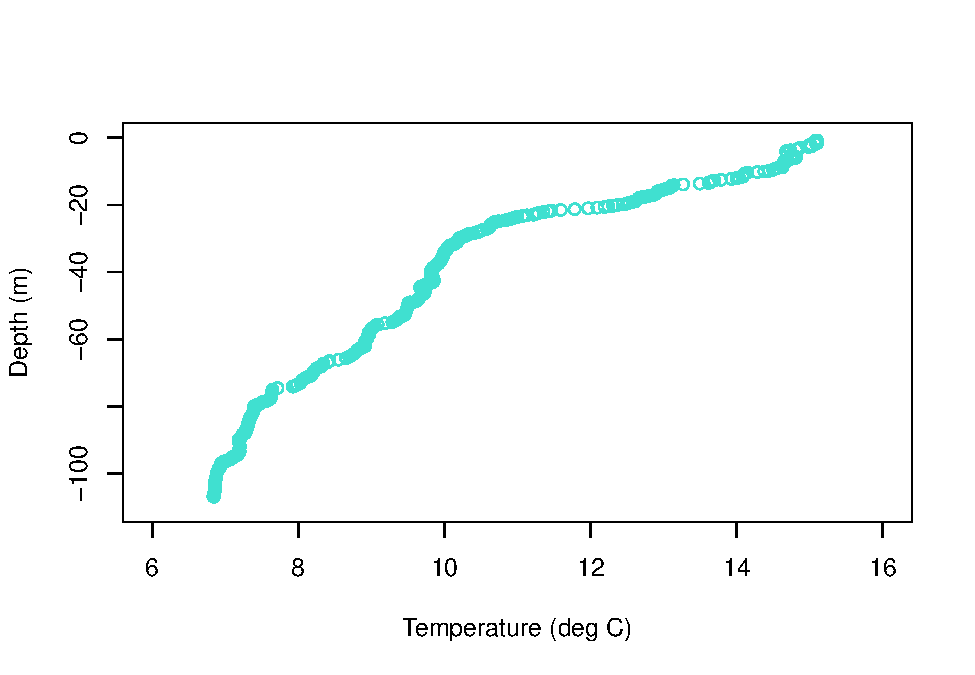
\includegraphics{dataVisualization-classNotes_files/figure-latex/unnamed-chunk-14-1.pdf}

\hypertarget{save-the-figure}{%
\paragraph{Save the figure}\label{save-the-figure}}

Type the following in your script

\begin{Shaded}
\begin{Highlighting}[]
\KeywordTok{png}\NormalTok{(}\StringTok{'temperature-station4-20170912.png'}\NormalTok{)}
\KeywordTok{plot}\NormalTok{(DATA[[}\StringTok{'Temperature.C'}\NormalTok{]],}\OperatorTok{-}\NormalTok{DATA[[}\StringTok{'Depth.m'}\NormalTok{]],}
 \DataTypeTok{xlab=}\StringTok{'Temperature (deg C)'}\NormalTok{,}\DataTypeTok{ylab=}\StringTok{'Depth (m)'}\NormalTok{,}
 \DataTypeTok{xlim=}\KeywordTok{c}\NormalTok{(}\DecValTok{6}\NormalTok{,}\DecValTok{16}\NormalTok{),}\DataTypeTok{ylim=}\KeywordTok{c}\NormalTok{(}\OperatorTok{-}\DecValTok{110}\NormalTok{,}\DecValTok{0}\NormalTok{),}
 \DataTypeTok{type=}\StringTok{"b"}\NormalTok{,}\DataTypeTok{col=}\StringTok{"turquoise"}\NormalTok{)}
\KeywordTok{dev.off}\NormalTok{()}
\end{Highlighting}
\end{Shaded}

\begin{verbatim}
## pdf 
##   2
\end{verbatim}

edg \#\#\#\# Save your script

Make sure you save your script, so you can run it again!

\end{document}
